\PassOptionsToPackage{unicode=true}{hyperref} % options for packages loaded elsewhere
\PassOptionsToPackage{hyphens}{url}
%
\documentclass[]{article}
\usepackage{lmodern}
\usepackage{amssymb,amsmath}
\usepackage{ifxetex,ifluatex}
\usepackage{fixltx2e} % provides \textsubscript
\ifnum 0\ifxetex 1\fi\ifluatex 1\fi=0 % if pdftex
  \usepackage[T1]{fontenc}
  \usepackage[utf8]{inputenc}
  \usepackage{textcomp} % provides euro and other symbols
\else % if luatex or xelatex
  \usepackage{unicode-math}
  \defaultfontfeatures{Ligatures=TeX,Scale=MatchLowercase}
\fi
% use upquote if available, for straight quotes in verbatim environments
\IfFileExists{upquote.sty}{\usepackage{upquote}}{}
% use microtype if available
\IfFileExists{microtype.sty}{%
\usepackage[]{microtype}
\UseMicrotypeSet[protrusion]{basicmath} % disable protrusion for tt fonts
}{}
\IfFileExists{parskip.sty}{%
\usepackage{parskip}
}{% else
\setlength{\parindent}{0pt}
\setlength{\parskip}{6pt plus 2pt minus 1pt}
}
\usepackage{hyperref}
\hypersetup{
            pdftitle={Tipologia i Cicle de Vida de les Dades},
            pdfauthor={Autors: Carlos Gómez, Carlos Molina},
            pdfborder={0 0 0},
            breaklinks=true}
\urlstyle{same}  % don't use monospace font for urls
\usepackage[margin=1in]{geometry}
\usepackage{graphicx,grffile}
\makeatletter
\def\maxwidth{\ifdim\Gin@nat@width>\linewidth\linewidth\else\Gin@nat@width\fi}
\def\maxheight{\ifdim\Gin@nat@height>\textheight\textheight\else\Gin@nat@height\fi}
\makeatother
% Scale images if necessary, so that they will not overflow the page
% margins by default, and it is still possible to overwrite the defaults
% using explicit options in \includegraphics[width, height, ...]{}
\setkeys{Gin}{width=\maxwidth,height=\maxheight,keepaspectratio}
\setlength{\emergencystretch}{3em}  % prevent overfull lines
\providecommand{\tightlist}{%
  \setlength{\itemsep}{0pt}\setlength{\parskip}{0pt}}
\setcounter{secnumdepth}{0}
% Redefines (sub)paragraphs to behave more like sections
\ifx\paragraph\undefined\else
\let\oldparagraph\paragraph
\renewcommand{\paragraph}[1]{\oldparagraph{#1}\mbox{}}
\fi
\ifx\subparagraph\undefined\else
\let\oldsubparagraph\subparagraph
\renewcommand{\subparagraph}[1]{\oldsubparagraph{#1}\mbox{}}
\fi

% set default figure placement to htbp
\makeatletter
\def\fps@figure{htbp}
\makeatother

\usepackage{etoolbox}
\makeatletter
\providecommand{\subtitle}[1]{% add subtitle to \maketitle
  \apptocmd{\@title}{\par {\large #1 \par}}{}{}
}
\makeatother

\title{Tipologia i Cicle de Vida de les Dades}
\providecommand{\subtitle}[1]{}
\subtitle{Pràctica 1 - Web Scraping}
\author{Autors: Carlos Gómez, Carlos Molina}
\date{Abril 2020}

\begin{document}
\maketitle

{
\setcounter{tocdepth}{1}
\tableofcontents
}
\begin{center}\rule{0.5\linewidth}{\linethickness}\end{center}

\hypertarget{context}{%
\section{1. Context}\label{context}}

\hypertarget{explicar-en-quin-context-sha-recollectat-la-informaciuxf3.-explicar-per-quuxe8-el-lloc-web-triat-proporciona-aquesta-informaciuxf3.}{%
\subsubsection{Explicar en quin context s'ha recol·lectat la informació.
Explicar per què el lloc web triat proporciona aquesta
informació.}\label{explicar-en-quin-context-sha-recollectat-la-informaciuxf3.-explicar-per-quuxe8-el-lloc-web-triat-proporciona-aquesta-informaciuxf3.}}

S'ha decidit fer aquesta pràctica de Web Scraping sobre Stadia, una nova
plataforma de videojocs en streaming de Google.

La idea d'agafar aquesta plataforma de videojocs va néixer en veure que
no existia cap lloc web on informes sobre l'evolució dels preus dels
jocs dins d'aquesta plataforma, cosa que seria interessant per veure si
en el moment de comprar un joc és una bona oferta o no. Ni la mateixa
empresa de Google dona aquesta informació en obert (sense estar
registrat), ni mitjançant la seva API. Suposem que en tractar-se d'una
plataforma bastant nova, no han implementat encara aquesta API.

A part de fer un seguiment dels preus dels jocs, també es interessant
poder extreure el llistat complet dels jocs que ja hi han a la
plataforma i els que estan confirmats que vindran en un futur. En
l'àmbit dels videojocs hi han moltes preguntes sobre la plataforma i
quins jocs són els que hi han. En tractar-se d'una plataforma tancada
als subscriptors ``PRO'', els usuaris normals només es poden informar
d'un llistat de jocs que hi ha a la web oficial de Stadia, però hem vist
que no son tots els que hi han actualment dins la plataforma. Això ho
hem pogut saber perquè un dels membres de l'equip té accés a la
plataforma desde dins, cosa que volem aprofitar per extreure la
informació dels jocs existents i fer un dataset amb aquesta informació.

Fins al dia 8 d'Abril de 2020, era una plataforma tancada als
subscriptors de pagament, on només els primers inscrits, al mes de
novembre, tenien accés. Ara mateix, s'ha obert aquest servei per a
tothom amb un compte de Google. Pel que es pot utilitzar qualsevol
compte per fer funcionar el script de scraping creat.

Per tant, en una primera fase ens hem marcat l'objectiu de:

\begin{itemize}
\tightlist
\item
  Obtenir un llistat amb tots el jocs disponibles i futurs, obtenint la
  informació de pàgines webs oficials.
\item
  Anar a buscar dades sobre aquests videojocs a altres webs per
  complementar la informació disponible i donar més valor al dataset.
  Dades com la puntuació a altres plataformes i dates de llançament.
\end{itemize}

\hypertarget{definir-un-tuxedtol-pel-dataset}{%
\section{2. Definir un títol pel
dataset}\label{definir-un-tuxedtol-pel-dataset}}

\hypertarget{triar-un-tuxedtol-que-sigui-descriptiu.}{%
\subsubsection{Triar un títol que sigui
descriptiu.}\label{triar-un-tuxedtol-que-sigui-descriptiu.}}

\textbf{Stadia Games Info}

Es tracta d'un llistat, on cada registre es un videojoc, o complement, i
s'amplia amb els atributs que donen informació sobre aquest videojoc.

\hypertarget{descripciuxf3-del-dataset}{%
\section{3. Descripció del dataset}\label{descripciuxf3-del-dataset}}

\hypertarget{desenvolupar-una-descripciuxf3-breu-del-conjunt-de-dades-que-sha-extret-uxe9s-necessari-que-aquesta-descripciuxf3-tingui-sentit-amb-el-tuxedtol-triat.}{%
\subsubsection{Desenvolupar una descripció breu del conjunt de dades que
s'ha extret (és necessari que aquesta descripció tingui sentit amb el
títol
triat).}\label{desenvolupar-una-descripciuxf3-breu-del-conjunt-de-dades-que-sha-extret-uxe9s-necessari-que-aquesta-descripciuxf3-tingui-sentit-amb-el-tuxedtol-triat.}}

\hypertarget{representaciuxf3-gruxe0fica}{%
\section{4. Representació gràfica}\label{representaciuxf3-gruxe0fica}}

\hypertarget{presentar-una-imatge-o-esquema-que-identifiqui-el-dataset-visualment}{%
\subsubsection{Presentar una imatge o esquema que identifiqui el dataset
visualment}\label{presentar-una-imatge-o-esquema-que-identifiqui-el-dataset-visualment}}

La primera imatge es una captura de la web interna de Stadia on pots
comprar els videojocs. Es pot observar que d'aquesta web podem obtenir
el títol, preu i tipus de joc:

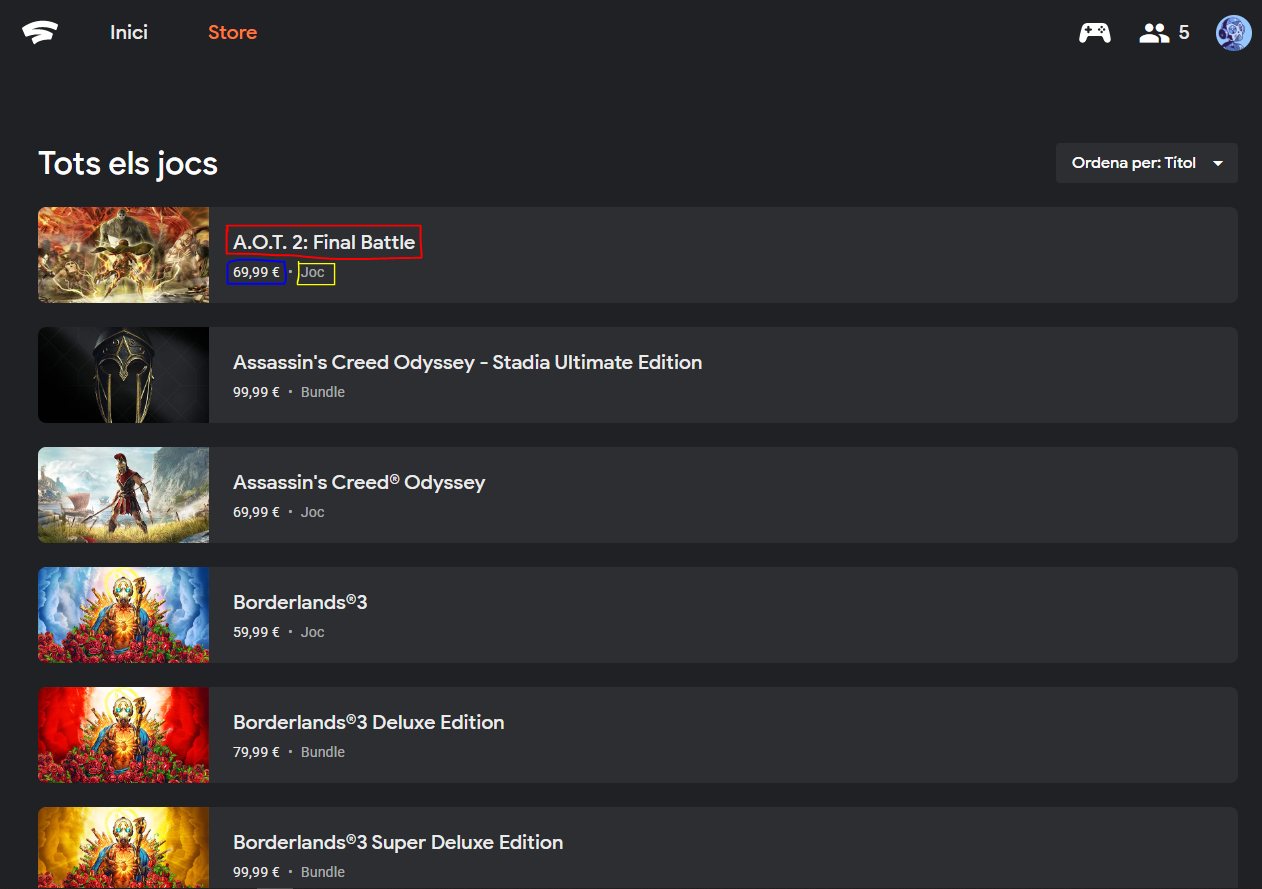
\includegraphics{stadia_store_list.png}

La segona web on anar a buscar informació és la pàgina on pots
inscriure't a la plataforma. En una de les pestanyes de la web pots
veure un llistat de jocs que anuncien:
\url{https://store.google.com/es/product/stadia_games}

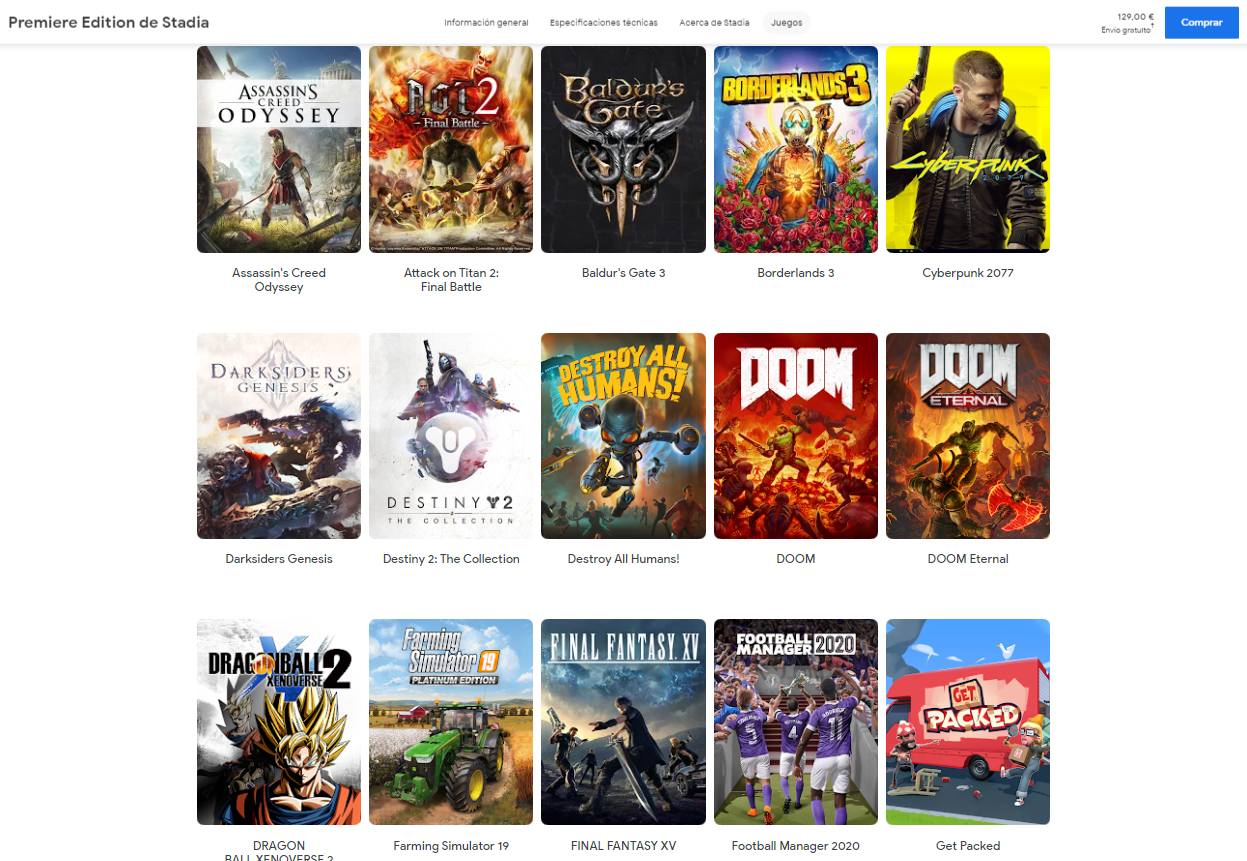
\includegraphics{store_google_stadia_games.png}

\hypertarget{contingut}{%
\section{5. Contingut}\label{contingut}}

\hypertarget{explicar-els-camps-que-inclou-el-dataset-el-peruxedode-de-temps-de-les-dades-i-com-sha-recollit.}{%
\subsubsection{Explicar els camps que inclou el dataset, el període de
temps de les dades i com s'ha
recollit.}\label{explicar-els-camps-que-inclou-el-dataset-el-peruxedode-de-temps-de-les-dades-i-com-sha-recollit.}}

\hypertarget{agrauxefments}{%
\section{6. Agraïments}\label{agrauxefments}}

\hypertarget{presentar-el-propietari-del-conjunt-de-dades.-uxe9s-necessari-incloure-cites-de-recerca-o-anuxe0lisis-anteriors-si-nhi-ha.}{%
\subsubsection{Presentar el propietari del conjunt de dades. És
necessari incloure cites de recerca o anàlisis anteriors (si n'hi
ha).}\label{presentar-el-propietari-del-conjunt-de-dades.-uxe9s-necessari-incloure-cites-de-recerca-o-anuxe0lisis-anteriors-si-nhi-ha.}}

\hypertarget{inspiraciuxf3}{%
\section{7. Inspiració}\label{inspiraciuxf3}}

\hypertarget{explicar-per-quuxe8-uxe9s-interessant-aquest-conjunt-de-dades-i-quines-preguntes-es-pretenen-respondre.}{%
\subsubsection{Explicar per què és interessant aquest conjunt de dades i
quines preguntes es pretenen
respondre.}\label{explicar-per-quuxe8-uxe9s-interessant-aquest-conjunt-de-dades-i-quines-preguntes-es-pretenen-respondre.}}

Existeixen webs semblants, que extreuen un llistat dels jocs disponibles
a la plataforma. Però, aquests portals estan mantinguts a mà pel seu
creador i no informen sobre el preu dels jocs:

\begin{itemize}
\tightlist
\item
  Stadia Game DB ---\textgreater{} \url{https://stadiagamedb.com/}
\item
  The Stadia DB ----\textgreater{} \url{thestadiadb.com}
\end{itemize}

La idea d'aquesta pràctica es poder tenir un script automatic que
obtingui tota aquesta informació en el moment d'executar-lo.

Una de les utilitats que pot tenir aquest script és la de extreure la
informació diariament, programant aquest script perque s'executi un cop
al dia. D'aquesta manera es podria fer un seguiment dels preus dels
videojocs a nivell individual i poder arribar a fer les visualitzacions
oportunes sobre aquesta informació.

\hypertarget{llicuxe8ncia}{%
\section{8. Llicència}\label{llicuxe8ncia}}

\hypertarget{seleccionar-una-daquestes-llicuxe8ncies-pel-dataset-resultant-i-explicar-el-motiu-de-la-seva-selecciuxf3}{%
\subsubsection{Seleccionar una d'aquestes llicències pel dataset
resultant i explicar el motiu de la seva
selecció:}\label{seleccionar-una-daquestes-llicuxe8ncies-pel-dataset-resultant-i-explicar-el-motiu-de-la-seva-selecciuxf3}}

Per aquest conjunt de dades hem escollit una llicència de Cultura
Lliure: \textbf{\emph{Reconeixement-CompartirIgual 4.0 Internacional de
Creative Commons}}

\begin{figure}
\centering
\includegraphics{https://i.creativecommons.org/l/by-sa/4.0/88x31.png}
\caption{CC BY-SA 4.0 License}
\end{figure}

\begin{itemize}
\tightlist
\item
  \textbf{BY:} Amb aquest tipus de llicència es dóna llibertat per
  copiar, reproduir o modificar el codi, sempre que es reconegui
  l'autoria del projecte original, per donar valor a la feina feta en
  aquesta pràctica.
\item
  \textbf{SA:} També afegim que els projectes derivats d'aquests, es
  comparteixin de la mateixa manera, per evitar que un producte derivat
  d'aquest tingui una llicència que prohibeixi l'ús comercial, limitant
  així les possibilitats de qualsevol persona que vulgui desenvolupar
\end{itemize}

\hypertarget{codi}{%
\section{9. Codi}\label{codi}}

\hypertarget{adjuntar-el-codi-amb-el-qual-sha-generat-el-dataset-preferiblement-en-python-o-alternativament-en-r.}{%
\subsubsection{Adjuntar el codi amb el qual s'ha generat el dataset,
preferiblement en Python o, alternativament, en
R.}\label{adjuntar-el-codi-amb-el-qual-sha-generat-el-dataset-preferiblement-en-python-o-alternativament-en-r.}}

El codi:

\begin{verbatim}
var = value
\end{verbatim}

\hypertarget{dataset}{%
\section{10. Dataset}\label{dataset}}

\hypertarget{publicar-el-dataset-en-format-csv-a-zenodo-amb-una-xicoteta-descripciuxf3.}{%
\subsubsection{Publicar el dataset en format CSV a Zenodo amb una
xicoteta
descripció.}\label{publicar-el-dataset-en-format-csv-a-zenodo-amb-una-xicoteta-descripciuxf3.}}

\hypertarget{lliurar}{%
\section{11. Lliurar}\label{lliurar}}

\hypertarget{presentar-el-treball-amb-el-doi-del-dataset-a-github}{%
\subsubsection{Presentar el treball amb el DOI del dataset a
Github}\label{presentar-el-treball-amb-el-doi-del-dataset-a-github}}

Tota la informació es pot trobar al repository de Github:
\url{https://github.com/KRLSMolina/ScrapingStadia}

\end{document}
